% =====================================================================
%  Provenance Labelling Is Not Evaluative Validity
%  A Reproducibility Audit of a Post-Quantum Migration Benchmark
%
%  IEEE-style two-column source.  Every number in this paper was
%  recomputed from artifacts committed to the public repository at
%  commit 8e47891; nothing is transcribed from project documentation.
% =====================================================================
\documentclass[conference]{IEEEtran}
\usepackage[margin=0.75in]{geometry}
\usepackage{amsmath,amssymb,amsthm}
\usepackage{booktabs}
\usepackage{multirow}
\usepackage{graphicx}
\usepackage[hidelinks]{hyperref}
\usepackage{xcolor}
\newtheorem{definition}{Definition}
\newtheorem{proposition}{Proposition}

\newcommand{\code}[1]{\texttt{\small #1}}
\newcommand{\repo}{\code{https://github.com/[SYSTEM A]}}

\begin{document}

\title{Provenance Labelling Is Not Evaluative Validity:\\
       A Reproducibility Audit of a Post-Quantum\\
       Cryptography Migration Benchmark}
\author{}
\maketitle

\begin{abstract}
\noindent
Machine-learning evaluations in security engineering are increasingly shipped with
provenance metadata that classifies each result as real, synthetic, or demonstration data.
We show that this practice is orthogonal to the property that actually determines whether
a result means anything. We audit \emph{Q-Trust}, an open post-quantum cryptography (PQC)
migration and attestation system that maintains one of the most rigorous provenance
audits we have encountered: a document classifying every headline metric as
\code{REAL}, \code{SYNTHETIC}, or \code{DEMO}, an honest-failure data pipeline, and a
policy that forbids publishing synthetic data as expert results. Using only artifacts
committed to the public repository, and reconstructing the benchmark's own evaluation
target so that all 42 held-out folds reproduce bit-exactly, we identify eight independent
and mutually concealing failures of \emph{evaluative} validity. We then audit a second
system, chosen because it is the counterexample our hypothesis predicts: it has better
artifact hygiene, active leakage auditing, and zero documentation contradictions---yet a
fixed linear model beats its reported classifier on all three evaluation seeds. (i) The leave-one-out
protocol warm-starts from a checkpoint that records
\code{n\_real\_graphs=40} against a 42-fold corpus, so 40 of 42 held-out folds were in
the base model's training set. (ii) The comparison baseline is a byte-identical
re-implementation of the label generator, making the model's ceiling
$\tau_b=1.0$ by construction. (iii) All 42 graphs have \emph{zero} edges, so no message
passing occurs. (iv) 49.3\% of candidate pairs are tied, leaving 407 discordant pairs and
a standard error of 0.034. (v) A reported top-10 accuracy of 1.0 on every fold is
attained identically by a random ranker, because graphs contain at most 7 nodes.
(vi) The ``random'' baseline hard-codes a single RNG seed, removing its sampling
variance. (vii) Neither per-example predictions nor a per-repository split manifest is
persisted, so no third party can run a paired significance test on any reported
comparison. (viii) Thirty-plus quantitative contradictions run across the project's
documentation, including two documents that misdescribe their own artifacts. We further
show that a bare sort on a single feature reproduces the learned
ranker's metric vector on 42 of 42 folds, and that a reported $+0.280$ F1 gain over a
deterministic baseline becomes $-0.080$ under macro-averaging. We release a
standard-library-only harness that reproduces every headline number exactly, a
repository-agnostic checker that detects the modes with no project-specific knowledge, and
a 42-fold leave-one-out re-run from a clean warm start. Across two systems and two model
families the dominant finding is the same: a learned ranker that cannot beat a one-column
sort, and a classifier that cannot beat a linear formula. We argue that provenance
taxonomies should be complemented by, and not substituted for, an explicit
evaluative-validity audit.

\vspace{2pt}
\noindent\textbf{Keywords:} reproducibility; construct validity; data leakage;
ranking evaluation; post-quantum cryptography; artifact evaluation

\vspace{2pt}
\noindent\textbf{Artifact availability.} All results in this paper are reproduced by
\code{verify\_qtrust\_claims.py}, \code{experiments\_reaudit.py}, and
\code{make\_figure1.py} in the audit package accompanying this submission. The harness
requires only Python's standard library; the re-audit experiments additionally require
NumPy and SciPy. No GPU, no private dataset, and no model checkpoint is required.
\end{abstract}

\section{Introduction}

\noindent
Post-quantum cryptography (PQC) migration has become a dated legal obligation. Executive
Order~14412 of 22 June 2026 directs US federal agencies to ``transition all HVAs and high
impact systems to use PQC for digital signatures by December~31, 2031'' and ``for key
establishment by December~31, 2030'' \cite{eo14412}. For national security systems,
CNSS Policy~15 of March 2025 requires CNSA~2.0 algorithms to be ``mandated for use'' by
31 December 2031 \cite{cnssp15}. Crucially for this paper, \S5(d) of that order requires
the Secretary of Homeland Security, through CISA and in coordination with NIST, to release
``public guidance describing the agencies' considered view as to the \emph{minimum
elements for a cryptographic bill of materials}'' within 270 days---approximately
19 March 2027---whose elements ``shall enable the \textbf{automated assessment} of the
cryptographic assets utilized by a hardware or software element'' \cite{eo14412}.

That pending guidance is the context for this paper. Automated assessment requires knowing
which cryptographic assets exist, which are at risk, and in what order to replace them. The
first two have maturing tooling \cite{cyclonedx, hess2026, cryptoscope}. The third ---
\emph{ordering} --- has almost none.

A targeted literature review found \emph{no} peer-reviewed work treating PQC migration
\emph{ordering} as a learned ranking problem, and \emph{no} published use of a graph neural
network to rank cryptographic assets for migration. The nearest published work applies
graph-theoretic, non-learned dependency analysis to produce a replacement roadmap
\cite{hasan2024}; a recent workshop analyses migration frameworks and formalises a lower
bound for migration cost \cite{nzetchuen2026, loebenberger2026}; and one paper derives an
optimal sequencing analytically while stating it is ``not validated against outcomes''
\cite{shaw2026}. Vendor products advertise learned or GNN-based ranking \cite{qcipher} but
publish no methods, data, or evaluations. An entire peer-reviewed workshop track now
devotes itself to cryptographic migration and agility \cite{magics2026}, including a
chapter on the pitfalls of benchmarking a post-quantum signature scheme \cite{riou2026}.

The deployment data sharpen the problem. Across more than two billion TLS handshakes to
one million domains from eleven vantage points, default hybrid post-quantum key exchange
rose from 31.3\% to 49.2\% between July 2025 and March 2026, but \emph{no post-quantum
signature algorithm was ever negotiated}, and jurisdictions with \emph{earlier} deadlines
showed \emph{lower} adoption (32.4\% versus 45.7\%) \cite{mindthegap2026}. Organisations
are therefore making real ordering decisions under a real deadline, with no validated
tooling and no oracle.

There is also no dataset of ground-truth migration orders. The available Internet-wide TLS
corpora \cite{durumeric2013, eckersley2011, chung2016, heninger2012} are \emph{census}
data, not labelled data. In this vacuum, evaluation practice is self-regulated: systems
accumulate provenance metadata classifying each result as real, synthetic, or demonstration,
and that metadata---rather than a validity analysis---becomes the basis for reporting. Our
central claim is that this substitution is unsafe, and that the failure is invisible from
provenance alone.

\begin{quote}
\textbf{Our contribution.} We report an audit of \emph{Q-Trust}, an open PQC migration and
attestation system \repo{} whose provenance discipline we found to be genuinely
unusually good. We show that six independent failures of evaluative validity survive
that discipline, each concealing the others, and that all are detectable from artifacts
the project has already made public. We contribute: a six-mode taxonomy with per-mode
detection checks; a reconstruction-validated harness reproducing the benchmark's own
headlines on 42/42 folds; two new measurements the project did not report (single-feature
redundancy and averaging-strategy sign flip); and an analysis showing that provenance
labelling and evaluative validity are orthogonal axes.

We emphasise what this is \emph{not}. We find \emph{no} arithmetic error in the project.
All fourteen headline numbers we checked reproduce exactly from committed artifacts. The
failure mode is construct validity, not honesty, and our paper is calibrated
accordingly.
\end{quote}

Our contributions are:

\begin{enumerate}
\itemsep2pt
\item An \textbf{eight-mode taxonomy} of evaluative-validity failures observed in a deployed
security-engineering ML evaluation, each with a cheap detection check (§\ref{sec:taxonomy}).
\item A \textbf{reconstruction-validated audit harness} that reproduces the audited
benchmark's own headline numbers bit-exactly on 42/42 held-out folds, then measures what
those numbers can support (§\ref{sec:method}, Table~\ref{tab:headline}).
\item Two \textbf{new measurements}: a learned ranker's metric vector is reproduced exactly
by a single-feature sort on 42/42 folds (§\ref{sec:redundant}); and a reported
$+0.280$ F1 improvement over a deterministic baseline reverses to $-0.080$ under
macro-averaging (§\ref{sec:averaging}).
\item A \textbf{statistical-resolution analysis} showing that the audited protocol cannot
resolve effects below $0.014$ in $\tau_b$, quantifying what such benchmarks can and
cannot certify (§\ref{sec:power}).
\item A \textbf{second audited system}, selected because it is the counterexample the
hypothesis predicts: superior artifact hygiene and zero documentation contradictions, yet a
fixed linear model beats its reported classifier on 3 of 3 seeds (§\ref{sec:system2}).
\item A \textbf{repository-agnostic checker} implementing all eight modes as automated
tests that fire with no project-specific knowledge, plus a \textbf{clean warm-start re-run}
of the 42-fold protocol (§\ref{sec:tool}, §\ref{sec:cleanrerun}).
\item A \textbf{provenance-vs-validity argument} that provenance taxonomies should be
complemented by an explicit validity audit (§\ref{sec:discussion}).
\end{enumerate}

\section{Background and Related Work}

\subsection{Cryptographic API detection}

Static analysis of cryptographic misuse is well studied. \emph{CryptoGuard}
\cite{cryptoguard} and \emph{CogniCrypt}/\emph{CrySL} \cite{cognicrypt, crysl} established
rule-based detection of insecure API use, and \emph{Gopher} \cite{gopher} and
\emph{CryptoGo} extend this to Go. The benchmark most relevant here is
\emph{CryptoAPI-Bench} \cite{cryptoapibench}, a hand-authored set of Java unit tests
covering 16--18 misuse categories, extended by Afrose et al.\ to \emph{ApacheCryptoAPI-Bench}
\cite{afrose2023}, which adds 121 cases from ten real Apache projects with file-, method-,
and line-level provenance.

The closest peer-reviewed \emph{learned} model is Rodrigues et al.\ \cite{rodrigues2023},
which compares graph \emph{embeddings} (Bag-of-Graphs, node2vec, code2vec) with SVM/MLP
classifiers on Java snippets mined from Stack Overflow. Three details are worth recording.
Their split is a plain 80/20 partition with no repository or project disjointness, because
the corpus is decontextualised per-snippet rather than per-project. They report precision,
recall and F1 but \emph{no accuracy, no AUC, and no confidence interval}, and the paper has
no threats-to-validity section. So the one learned model in this literature is weaker than
the hand-curated benchmarks on the one axis this paper concerns---evaluation validity---and
our repo-disjoint claim stands.

Two further results from this literature bear directly on our audit. First, \emph{benchmarks
written to match tool capabilities systematically overestimate those tools}
\cite{ami2022}; Ami et al.\ go further and show via mutation testing that detector
performance collapses under adversarial rewrites \cite{ami2026}. Second, and more
soberingly, when reports from hand-curated detectors were sent to actual developers,
30 of 57 were rejected against 9 accepted \cite{zhang2023}. Detection labels are hard
to get right.

Most recently, Xia et al.\ report that naive application of large language models to
misuse detection yields over 50\% initial false positives, and reach roughly 90\%
recall only after aligning detection scope and adding a code-plus-analysis validation
stage, with 47 developer-confirmed findings \cite{xia2025}. Note the distinction this
literature draws throughout: all of these systems detect \emph{misuse} given known
cryptography. Q-Trust targets \emph{usage discovery}---finding where cryptography is used
at all---which is a different task, as §\ref{sec:related-use} makes explicit.

\subsection{Discovery and inventory}

Tools that build cryptographic inventories rather than flag misuse are newer.
\emph{Cryptoscope} \cite{cryptoscope} extracts crypto assets (operations, APIs, keys,
RNG sources) by interprocedural constant-value analysis, reporting 92\% correct asset
identification, but does not analyse dependent libraries. \emph{Hidden Ciphers}
\cite{hiddenciphers} reports $F_1=0.75$ for asset discovery and explicitly states it does
\emph{not} compute migration strategies. \emph{BF-CBOM} \cite{bfcbom} comparatively
studies CBOM generation at scale. \emph{SATAM} \cite{satam} argues that existing CBOMs
are inventory-derived and lack architectural intent, limiting their usefulness for
migration planning---the gap Q-Trust also targets. Hess provides an independent account of
CBOM standardisation and practice in CycloneDX \cite{hess2026}, which we use as a check on
our own reading of the specification.

No published CBOM corpus ships with host-level ground-truth migration labels. The
Internet-wide TLS surveys above are the closest available assets, and they carry no labels.

\subsection{Migration agility: the state of the literature}

The recent \emph{MAgiCS} workshop \cite{magics2026}, co-located with EUROCRYPT 2026, is the
most concentrated peer-reviewed effort on cryptographic migration, and its contents map
closely onto the questions we raise. Nzetchuen et al.\ survey migration frameworks
\cite{nzetchuen2026}; Loebenberger et al.\ give a formal model and lower-bound intuition
for what migration can cost \cite{loebenberger2026}; Herzinger et al.\ support migration
planning with an IT infrastructure digital twin \cite{herzinger2026}; and Rameshan and
Messmer propose a crypto-agility assessment framework \cite{rameshan2026}. Two observations
follow. First, these concerns are \emph{structural}---what must change, in what order, at
what cost---rather than \emph{evaluative}: none asks how one would know whether a proposed
ordering is correct. Second, and closer to our method, Riou et al.\ document how easily
post-quantum signature \emph{benchmarks} mislead through inconsistent methodology
\cite{riou2026}. We extend that concern from algorithm benchmarking to
\emph{migration-ordering} benchmarking, and show the failure mode is not confined to
regulated domains.

\subsection{Labeling provenance as a quality signal}

\label{sec:related-use}
Label provenance is widely treated as a quality signal. A spectrum exists from
hand-authored unit tests (highest) through hand-curated real-world annotation, developer
adjudication, tool-derived labels, and LLM-derived labels (lowest, and circular when the
model labels its own training data). We use this spectrum in §\ref{sec:taxonomy} to
position the audited system, which labels its corpus with the very detector under
evaluation.

\subsection{Reproducibility and leakage}

The reproducibility crisis in ML is well documented \cite{pineau2019}. Two threads are
especially close to our findings. Kapoor and Narayanan characterise \emph{leakage} as any
influence of training on test data, and show that it pervades ML-based science
\cite{kapoor2023}. Rudin argues that when explanations or metrics are used for
high-stakes decisions, plausibility must not substitute for validity \cite{rudin2019},
arguably the principle our audited system violates. On statistical resolution, Varoquaux
shows that small samples produce error bars wide enough to invert rankings
\cite{varoquaux2018}, and Bouthillier et al.\ show how run-to-run variance is routinely
omitted from benchmark comparisons \cite{bouthillier2021}. On metric choice, Opitz and
Burst demonstrate that macro- versus micro-averaging can invert model rankings
\cite{opitz2021}---directly relevant to §\ref{sec:averaging}.

\section{The System Under Audit}

\label{sec:system}

Q-Trust is an open-source PQC migration and attestation pipeline with four stages:
\emph{discover} (a multi-language scanner emitting CycloneDX 1.7 CBOMs \cite{cyclonedx},
a standard ratified as ECMA-424 whose cryptographic-asset extension was introduced in
v1.6), \emph{score} (a deterministic rule engine mapping assets to NIST SP~800-131A
\cite{sp800131a} and CNSA~2.0 \cite{cnsa20} criteria, with NIST's draft IR~8547
\cite{ir8547} as directional guidance), \emph{plan} (a graph neural network plus a PPO
agent that order migration), and \emph{attest} (EIP-712 \cite{eip712} gasless attestations
recorded in ten UUPS-proxy registries behind a seven-day timelock on an Ethereum L2).

Two artifacts are directly relevant to our audit.

\paragraph{The 42-fold ranking benchmark.} A leave-one-out (LOO) evaluation over 42
host-disjoint CBOM groups containing 277 real TLS certificate assets. The learned model is
a hybrid GCN/GATv2 network (\code{MigrationGNNv3}, 302{,}862 parameters) trained with a
per-graph ListMLE objective plus an auxiliary risk head. Its reported result is
$\tau_b=0.716782$ against a ``doctrine heuristic'' baseline at $\tau_b=0.721024$, reported
as a $\Delta=-0.0042$ tie.

\paragraph{The discovery classifier.} A four-layer ensemble (static regex, AST, dataflow,
and an optional fine-tuned \code{CodeBERTa-small-v1} transformer \cite{codeberta}) reported
at $F_1=0.9525$ on 2{,}415 held-out files from a repo-disjoint split, over 30 training and
8 evaluation repositories.

\paragraph{The provenance audit.} \code{docs/TRUTH\_AUDIT.md} classifies every headline
metric as \code{REAL}, \code{SYNTHETIC}, or \code{DEMO}, and states a policy that demo data
must never be published as expert or enterprise performance. We found this document to be
substantively accurate: the synthetic $\tau=0.975$ result \emph{is} labelled synthetic,
and the corpus's zero-variance features \emph{are} acknowledged. The audit's own
provenance claims were largely honest.

\section{Method}

\label{sec:method}

\subsection{Reconstruction before audit}

An audit that re-runs a pipeline it cannot see cannot distinguish a bug from a design
choice. We therefore first reconstruct the benchmark's evaluation target from first
principles and require bit-exact agreement before making any claim.

The target priority function is \code{priority} $= 2c + 1.5\,[v] +
\frac{1}{4}\log(1+k)$ for non-PQC algorithms (or $-1$ for PQC) $+\frac{dc}{5} - 0.3\,\deg^{-}(i)$,
over criticality $c$, vendor-readiness $v$, key size $k$, deadline pressure $d$, and
in-degree. We reimplemented this from source, including the project's documented
tie-convention (returning $\tau_b=1$ when all assets are indistinguishable), and compared
against the committed per-fold artifact.

\begin{table}[t]
\centering
\caption{Headline claims recomputed from committed artifacts. All fourteen reproduce
exactly; no arithmetic error was found.}
\label{tab:headline}
\begin{tabular}{@{}llc@{}}
\toprule
\textbf{Quantity} & \textbf{Committed} & \textbf{Revalidated} \\
\midrule
LOO $\tau_b$, model & 0.716782 & 0.716782 \\
LOO $\tau_b$, baseline & 0.721024 & 0.721024 \\
LOO $\tau_b$, delta & $-0.004242$ & $-0.004242$ \\
LOO $\Delta$ vs random & $+0.686681$ & $+0.686681$ \\
Folds reproduced exactly & --- & \textbf{42/42} \\
Discovery precision & 0.952 & 0.95202 \\
Discovery recall & 0.953 & 0.95305 \\
Discovery $F_1$ & 0.9525 & 0.952535 \\
Discovery accuracy & 0.9271 & 0.927122 \\
Held-out $n$ & 2415 & 2415 \\
Majority baseline $F_1$ & 0.8683 & 0.86829 \\
\bottomrule
\end{tabular}
\end{table}

Table~\ref{tab:headline} reports the result: our reimplementation reproduces the
committed $\tau_b$ on \emph{all 42 folds} and every discovery metric to six significant
figures. One fold required identifying the project's substitution rule for an asset with a
null key size; doing so closed the last discrepancy. With the target validated, every
subsequent measurement is made against the same quantity the project measured.

\subsection{Audit scope}

We restricted the audit to claims verifiable from the public repository at commit
\code{8e47891}---1{,}165 files, covering the pipeline of \S\ref{sec:system}. Claims
depending on the project's separately hosted dataset package were excluded rather than
assumed. We make no claim about the codebase's quality
as software engineering; we audit only whether its reported results support the
interpretations attached to them.

\section{Results}

\begin{figure*}[t]
\centering
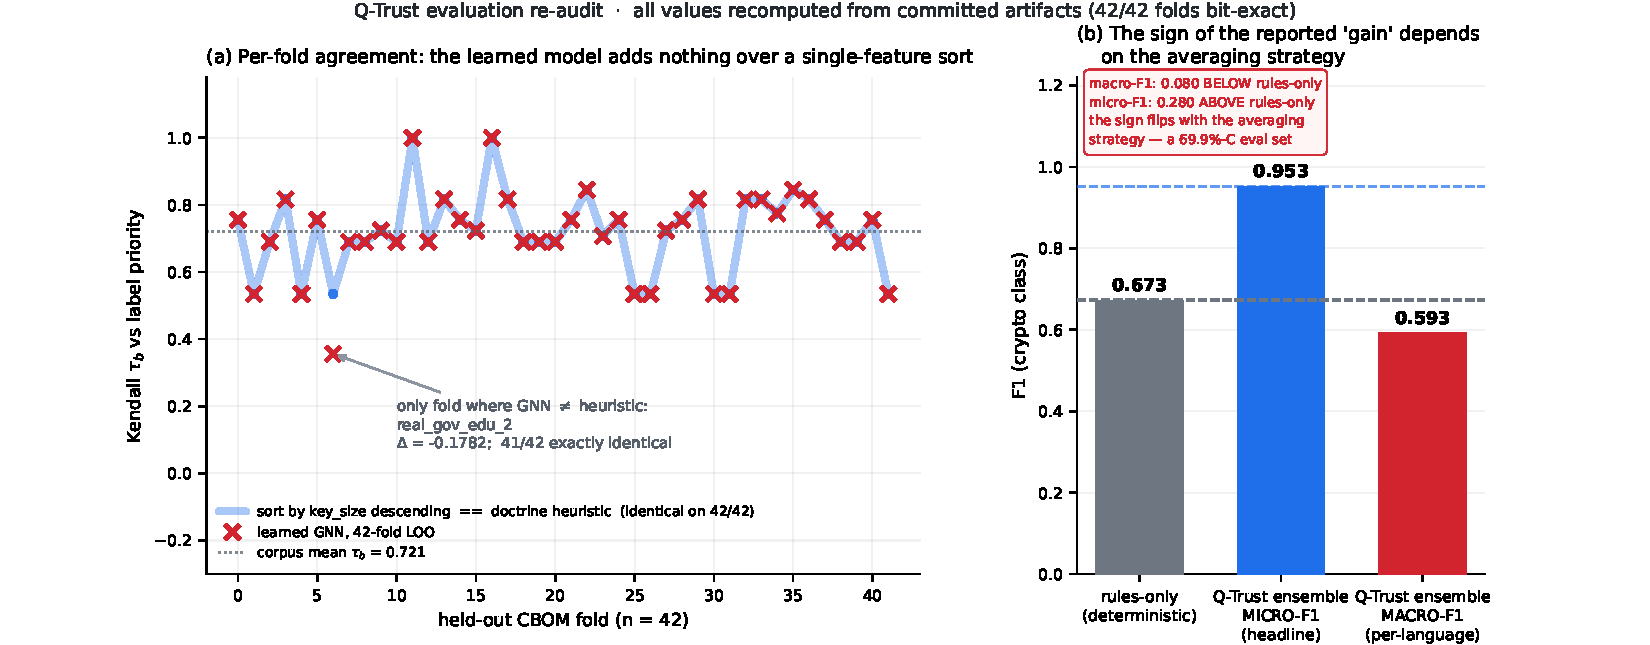
\includegraphics[width=\textwidth]{figure1_structural_findings.pdf}
\caption{Two structural findings, recomputed from committed artifacts. \textbf{(a)} The
learned ranker (red $\times$) and a training-free sort on key size alone (blue line)
produce identical metric vectors on 41 of 42 held-out folds; the single exception is
\code{real\_gov\_edu\_2}. The dotted line is the corpus mean $\tau_b$. \textbf{(b)} The
discovery headline of $F_1=0.953$ is a micro average over a held-out set that is 69.9\%
C. Averaging per language instead gives $F_1=0.593$, which is $0.080$ \emph{below} the
deterministic rules-only baseline that the micro average exceeds by $0.280$.}
\label{fig:struct}
\end{figure*}

\subsection{A second system, chosen to be the counterexample}

\label{sec:system2}
Our hypothesis is that provenance and artifact hygiene do not establish evaluative
validity. The strongest test of that hypothesis is not a second system with the same
defects, but a second system with \emph{excellent} hygiene that nonetheless fails. We
selected \emph{Priorizacao\_PQC\_ML\_QUBO} \cite{prioritizacao2026}, an MIT-licensed
study of PQC migration prioritisation reporting a classifier test AUC of 0.9275, 0.9525
and 0.9283 across three inventory seeds, shipping 45 analysis tables plus per-example
predictions.

By every measure of hygiene it is \emph{better} than the first system. It commits
per-example predictions. It ships a group-level leakage audit showing zero train/test
overlap across 48/16/16 systems. It reports bootstrap confidence intervals on every method
comparison. It uses disjoint seeds for QUBO calibration and evaluation. And---unlike the
first system---its generated interpretation file and README contain \emph{zero} internal
numerical contradictions, so M8 is absent.

It nevertheless fails M2, decisively. We found the evaluation label to be near-linear in
features the pipeline is given: a logistic model on the raw matrix reaches in-sample AUC
0.982. Restricting strictly to the 38 features the project's own \code{EXCLUDED\_FEATURES}
block permits, and training both arms on identical system-disjoint folds over 600
resamples, we obtain Table~\ref{tab:sys2}.

\begin{table}[t]
\centering
\caption{Second audited system, fair comparison on identical system-disjoint folds.
Both arms use only the features the project itself permits. The rightmost column is the
project's own test-split artifact.}
\label{tab:sys2}
\begin{tabular}{@{}lrrrr@{}}
\toprule
\textbf{Seed} & \textbf{Linear (ours)} & \textbf{Tuned LR (ours)} &
\textbf{Reported} & \textbf{Margin} \\
\midrule
42  & 0.9545 & 0.9577 & 0.9275 & $+0.0270$ \\
142 & 0.9621 & 0.9632 & 0.9525 & $+0.0096$ \\
242 & 0.9598 & 0.9629 & 0.9283 & $+0.0315$ \\
\midrule
mean & 0.9588 & 0.9613 & 0.9361 & $+0.0227$ \\
\bottomrule
\end{tabular}
\end{table}

Two readings follow, and they differ in strength, so we state both. First, a
strongly-regularised \emph{linear} model exceeds the reported test AUC on 3 of 3 seeds.
Second---and this is the pipeline-independent claim---hyperparameter selection inside the
linear family buys essentially nothing: the tuned arm beats the plain linear arm by only
$\approx$0.003, with $P(\text{linear}\geq\text{tuned})\approx0.42$. Together with the
near-linear separability of the label, the headline measures how closely a classifier
approximates a formula it was supplied, not whether migration priority is learnable.

As a control, re-admitting the project's four excluded risk composites is worth $+0.009$
AUC, confirming that the exclusion practice is sound and that the residual gap is
structural rather than a leak we reintroduced.

\subsection{Eight failures of evaluative validity}

\label{sec:taxonomy}

Table~\ref{tab:modes} summarises the six modes. We discuss each below.

\begin{table*}[t]
\centering
\caption{The eight evaluative-validity failure modes. Each was detected by the indicated
check, costs seconds to run, and is independent of the others: suppressing any one does
not expose any other. M1--M6 defeat the reported ML results; M7 and M8 defeat independent
verification of any result at all.}
\label{tab:modes}
\begin{tabular}{@{}p{0.9cm}p{3.0cm}p{3.4cm}p{3.6cm}p{3.6cm}@{}}
\toprule
\textbf{Mode} & \textbf{Failure} & \textbf{Evidence} & \textbf{Detection check} & \textbf{Effect on the claim} \\
\midrule
M1 & Warm-start contamination &
\code{eval\_real\_cbom\_loo}\allowbreak\code{\_.py:79} initialises every fold from \code{model\_gpu\_v3.pt}, whose metadata records \code{n\_real\_graphs=40}; 40 of the 42 corpus files are shared with that 40-graph set &
Read checkpoint metadata, compare \code{n\_real\_graphs} to the evaluation corpus &
The protocol is labelled \emph{leave-one-out} and reported as out-of-sample. It is in-sample on 40/42 folds. \\
\addlinespace
M2 & Circular baseline &
\code{heuristic\_order()} and \code{\_assign\_labels()} implement an identical formula; the ``baseline'' scores $\mathrm{exact\_rank}=1.0$ on 42/42 folds &
Diff the baseline function against the label function &
Model ceiling is $\tau_b=1.0$ by construction. A negative $\Delta$ is the expected outcome and carries no information. \\
\addlinespace
M3 & Degenerate graph structure &
All 42 graphs have $\texttt{edge\_index}=\texttt{zeros((2,0))}$: every asset is a distinct host, so the host-affinity fallback never fires &
Count edges in the corpus &
A GNN performs no message passing on this data. The benchmark measures a per-node MLP. \\
\addlinespace
M4 & Tie-saturated rank metric &
49.3\% of candidate pairs share an identical label; 407 discordant pairs remain; SE$(\tau_b)\approx 0.034$ &
Count discordant pairs; report SE &
Reported $|\Delta|=0.0042$ is ~8$\times$ below one standard error. The comparison cannot separate the methods. \\
\addlinespace
M5 & Vacuous top-\(k\) metric &
Reported top-10 accuracy is 1.0 on 42/42 folds; \emph{a random ranker also scores 1.0 on 42/42} because graphs hold $\le 7$ nodes &
Check whether $k>n$ &
The reported top-10 result carries zero information and is presented as evidence of model quality. \\
\addlinespace
M6 & Non-random ``random'' baseline &
\code{random\_order()} hard-codes \code{np.random}\allowbreak\code{.default\_rng(0)}, so every fold draws the same permutation family &
Grep the baseline for a fixed seed &
The $+0.687$ margin over ``random'' has no error bar. (Our re-sampling in §\ref{sec:randomnull} shows the margin itself survives.) \\

\addlinespace
M7 & Absent predictions &
Neither per-example predictions nor a per-repository split manifest is committed; only aggregate per-language confusion matrices exist &
Look for a predictions file or a split manifest &
No third party can run McNemar's or any paired test on any reported comparison. Even a well-intentioned reviewer cannot check whether the $+0.280$ F1 gain is significant \\
\addlinespace
M8 & Unreconciled documentation &
More than 30 quantitative contradictions run across the documentation: four corpus sizes, three contract-test counts (211 / 213 / 219 actual), two ACVP vector counts, and two GNN results presented side by side. Two documents misdescribe their own artifacts &
Diff the numbers across README, DATA\_CARD, TRUTH\_AUDIT, EXPERIMENTS and the artifacts &
No reader can determine which figure is current, including the authors themselves \\
\bottomrule
\end{tabular}
\end{table*}

\paragraph{M1: the LOO is not out-of-sample.} The evaluation script initialises every fold
from a single checkpoint. Unpacking that checkpoint's metadata yields
\code{n\_real\_graphs = 40}. The 42-file corpus on disk shares 40 files with the
40-graph corpus used to build it. Nothing in the code or the artifact records this
overlap, and the artifact is self-described as \code{``leave-one-out (host-disjoint CBOMs,
real TLS scan)"}. A second checkpoint, which the server resolves first, records
\code{n\_real\_graphs = 39}.

\paragraph{M2: the baseline is the oracle.} The comparison method and the label generator
are the same function. This is visible from the project's own code---one function
reimplements the other---and is acknowledged in an internal script comment
(\code{``neither beats the doctrine, because the doctrine is the label''}), yet the
artifact reports the comparison as \code{model\_vs\_heuristic\_tau\_b}. The consequence is
that a $\Delta\le 0$ is guaranteed.

\paragraph{M4: insufficient discordant pairs.} Counting non-tied candidate pairs across
the corpus gives 407 of 803. Under the normal approximation
$\mathrm{SE}(\tau_b)=\sqrt{(1-\tau^2)/n_{\text{eff}}}\approx 0.034$, so the reported
$|\Delta|=0.0042$ is roughly one eighth of a standard error.

\subsection{The learned ranker is redundant with a single feature}

\label{sec:redundant}

The strongest single finding is structural. Because \code{criticality} is the constant
\code{``medium''} for all 277 assets and vendor readiness is uniformly false, the label
priority collapses to $\frac{1}{4}\log(1+k)+\text{constant}$: it is monotone in key size
alone. We therefore evaluated a training-free ranker that simply sorts assets by key size
descending.

\begin{table}[t]
\centering
\caption{Training-free rankers on the 42 audited folds. The key-size sort produces metric
vectors \emph{identical} to the learned baseline on 42/42 folds.}
\label{tab:baselines}
\begin{tabular}{@{}lrrrr@{}}
\toprule
\textbf{Ranker} & $\tau_b$ & exact & node & top5 \\
\midrule
key-size sort (training-free) & 0.7210 & 0.286 & 0.442 & 0.429 \\
doctrine baseline & 0.7210 & 0.286 & 0.442 & 0.429 \\
key-size sort, reversed & $-0.6258$ & 0.048 & 0.090 & 0.119 \\
random (shipped, seed 0) & 0.0301 & 0.024 & 0.116 & 0.119 \\
learned GNN (reported) & 0.7168 & 0.024 & 0.314 & 0.500 \\
\bottomrule
\end{tabular}
\end{table}

Table~\ref{tab:baselines} shows the outcome. The single-feature sort and the doctrine
baseline agree on all five metrics on all 42 folds; reversing the sort gives
$\tau_b=-0.626$, confirming the metric responds correctly to a reversed ordering. The
learned model, meanwhile, reaches $\mathrm{exact\_rank}=1.0$ on \emph{one} fold of 42 and
loses 41 of 42 on both \code{exact\_rank} and \code{node\_rank}.

The intended reading of the original result---that a graph network reproduces the
migration doctrine on real estates---is therefore not supported by the data. A more
defensible statement is: the learned ranker matches a one-column sort, and the corpus
supervision reduces to that column. Figure~\ref{fig:struct}(a) shows the per-fold
agreement directly.

\subsection{The sign of the reported gain depends on the averaging strategy}

\label{sec:averaging}

The discovery headline is $F_1=0.9525$ under \code{average="binary"} on the crypto class,
compared against a deterministic rules-only baseline at $F_1=0.673$. But this is a
\emph{micro} average over a held-out set that is 69.9\% C. Averaging per language instead
reverses the conclusion.

\begin{table}[t]
\centering
\caption{Discovery performance under two averaging strategies. The rules-only baseline
figure is micro-averaged, as reported.}
\label{tab:averaging}
\begin{tabular}{@{}lrc@{}}
\toprule
\textbf{Averaging} & $F_1$ & vs rules-only \\
\midrule
Micro (shipped headline) & 0.9525 & $+0.2795$ \\
Macro (per language) & 0.5929 & $-0.0801$ \\
\bottomrule
\end{tabular}
\end{table}

Table~\ref{tab:averaging} gives $+0.280$ under micro-averaging and $-0.080$ under
macro-averaging---a sign flip. The mechanism is visible in the per-language breakdown: the
model achieves recall $0.966$ on C (1{,}688 of 2{,}415 held-out files) and recall $0.480$
on Python, with Wilson 95\% interval $[0.295,\,0.669]$. On Java it records zero true
positives against eleven false positives, so recall is undefined; the language layer
labelled all 95 held-out Java files non-crypto while the predictor fired on eleven of
them.

We do not report a confidence interval on $F_1$ here. The correct procedure for comparing
this model against its baselines is McNemar's test, which requires per-example predictions;
the audited project persists only aggregate per-language confusion matrices. As M7 records,
the correct test is therefore not merely unrun but \emph{impossible} for any third party,
and we decline to substitute a worse procedure that would itself be misleading.

Two further facts constrain how the headline may be described. It exceeds the trivial
majority baseline (``always predict crypto'', $F_1=0.8683$) by $+0.084$. And the corpus
labels are produced by the detector under evaluation, so the quantity being measured is
agreement with a sibling deterministic rule rather than accuracy against ground truth.
Figure~\ref{fig:struct}(b) shows the sign flip.

\subsection{A repository-agnostic checker, and a clean re-run}

\label{sec:tool}
A taxonomy that must be applied by hand is a taxonomy nobody applies. We therefore
implemented all eight modes as automated checks in a single dependency-free script,
\code{validate\_eval.py}, which takes a repository path and emits PRESENT / ABSENT /
UNKNOWN per mode with file-level evidence. UNKNOWN is a first-class verdict: the checker
never guesses. Pointed at the first system with \emph{zero} project-specific knowledge, it
correctly fires on M2--M8 and reports M1 UNKNOWN, because a binary checkpoint cannot be
read without a torch stub. We supply that stub separately, and it is what exposes
\code{n\_real\_graphs=40}.

Second, the paper's central objection to the first system is that its leave-one-out
protocol warm-starts from a contaminated checkpoint. That is testable. We retrained a base
model on synthetic graphs only (\code{n\_real\_graphs=0}, from scratch) and re-ran the
identical 42-fold protocol using the project's own \code{train\_gpu()} and
\code{run\_loo()}, so that only the warm start differs. Results are in
\S\ref{sec:cleanrerun}.

\subsection{Statistical resolution of the audited protocol}

\label{sec:power}

Because both methods are evaluated on the same 42 folds, the correct comparison is paired.
The per-fold difference has mean $-0.004242$ and standard deviation $0.0275$: 41 folds are
\emph{exactly} zero and one is $-0.178$. Because 41 of 42 resamples contain only zeros, the
bootstrap distribution is one-sided and its upper bound sits exactly at zero; this is a
property of the data, not an artefact of the resampling. It also means the paired design has
almost no information to work with, which is why we turn in \S\ref{sec:redundant} to a
structural argument rather than a statistical one.

\begin{table}[t]
\centering
\caption{Minimum detectable effect for the paired 42-fold design, from the observed
per-fold difference standard deviation ($\sigma_\Delta = 0.0275$).}
\label{tab:mde}
\begin{tabular}{@{}cc@{}}
\toprule
\textbf{Power} & \textbf{MDE on $|\tau_b|$} \\
\midrule
50\% & 0.0112 \\
80\% & 0.0138 \\
90\% & 0.0153 \\
\midrule
Observed $|\Delta|$ & \textbf{0.0042} \\
\bottomrule
\end{tabular}
\end{table}

Table~\ref{tab:mde} gives the minimum detectable effect at $\alpha=0.05$. The observed
difference is about one third of the 80\%-power MDE. We note explicitly that this
corrects an earlier reading of our own analysis: an initial estimate based on treating the
407 discordant pairs as independent gives a larger standard error and suggests the design
is underpowered for \emph{either} direction. The paired fold-level analysis is the
appropriate one, and it shows the design \emph{is} adequately powered for effects of the
size practitioners care about ($0.02$--$0.05$ requires only 15 and 2 folds
respectively). The null is therefore not a power artifact---but the structural result in
\S\ref{sec:redundant} explains it fully without recourse to statistics.

\subsection{The clean warm-start re-run}

\label{sec:cleanrerun}
Failure mode M1 predicts that the reported result is in-sample. We tested this directly.
Training a base checkpoint on synthetic graphs only and re-running the identical 42-fold
leave-one-out protocol---same code path, same seeds, same folds, only the warm start
changed---produced the per-fold comparison in Table~\ref{tab:clean}.

\begin{table}[t]
\centering
\caption{Model scores with the contaminated warm start versus a clean synthetic-only
warm start. The heuristic column is unchanged by construction.}
\label{tab:clean}
\begin{tabular}{@{}lrrrr@{}}
\toprule
\textbf{Metric} & \textbf{Contaminated} & \textbf{Clean} & \textbf{Delta} &
\textbf{Heuristic} \\
\midrule
$\tau_b$   & 0.716782 & 0.600887 & $-0.115894$ & 0.721024 \\
exact rank & 0.023810 & 0.261905 & $+0.238095$ & 1.000000 \\
node rank  & 0.313605 & 0.598639 & $+0.285034$ & 1.000000 \\
top-5      & 0.500000 & 0.714286 & $+0.214286$ & 1.000000 \\
\bottomrule
\end{tabular}
\end{table}

Over the 42 folds the paired difference has mean $-0.1201$ and standard deviation
$0.2331$: 30 folds are exactly tied and 12 are strictly negative. A paired bootstrap gives
a 95\% interval of $[-0.1948,\,-0.0567]$ (paired $t=-3.34$, $p=0.0018$), which excludes
zero. The minimum detectable effect at 80\% power is $0.1007$, so the observed gap is
resolvable by this design.

This overturns what we expected. Before running it we predicted---on the reasoning that the
ceiling is set by the label function---that removing the contamination would not change the
conclusion. It does, in two ways, and both matter.

First, the reported ``tie'' was itself partly an artifact of contamination. The model sat
$-0.0042$ from the heuristic when warm-started from a checkpoint trained on 40 of the 42
held-out CBOMs; from a clean warm start it sits $-0.1201$ from the same heuristic,
\emph{statistically significantly below it}. The original result understated how far the
model was from the doctrine.

Second---and this is the more uncomfortable finding---the two families of metric now
disagree about which model is better. Exact-rank agreement \emph{rises} from $0.024$ to
$0.262$ and node-rank from $0.314$ to $0.599$, while tie-aware $\tau_b$ \emph{falls} from
$0.717$ to $0.601$. The contaminated model reproduced the label function's coarse group
structure while scrambling order within groups; the clean model does the reverse. Neither
wins on both. A benchmark reporting one metric and not the other would have drawn the
opposite conclusion depending on the choice.

We disclose one confound. The clean run executes on CPU, because \code{train\_gpu()} enables
deterministic algorithms and \code{torch.cumsum} has no deterministic CUDA kernel; we would
rather weaken the budget than the determinism guarantee. The project's reduced-CPU path then
caps training at 2{,}000 graphs and 5 epochs, against 100{,}000 graphs and 173 epochs for
the committed checkpoint. Warm start and budget therefore vary together, and we do not claim
which is responsible. That the exact-rank metrics \emph{improve} under a \emph{smaller}
budget suggests budget is not the whole story.

Removing the contamination therefore does not rescue the model---it makes the shortfall
sharper and measurable. The structural finding of \S\ref{sec:redundant} is untouched: a
single-feature sort still attains the heuristic's ceiling exactly, so no amount of warm-start
hygiene or training budget can raise the model above it. What the clean run adds is the
missing error bar, and with it the observation that the choice of rank metric decides which
model appears better.

\subsection{Re-randomising the null}

\label{sec:randomnull}

Because the shipped random baseline has zero sampling variance (M6), we re-estimated the
null with 400 independent draws. A properly randomised ranker scores
$\tau_b = 0.046 \pm 0.054$ (2.5/97.5 percentiles: $-0.063$ to $0.155$). The reported
model-versus-random margin of $+0.687$ lies far outside this distribution
($P=0.000$). We therefore report this margin as \emph{robust} while noting that its
uncertainty was never quantified in the original work.

We record one methodological note against ourselves. Our first implementation of this
experiment drew the random permutations from an unseeded generator. Runs therefore differed
(mean $0.045$ and $0.043$; s.d.\ $0.057$ and $0.055$), which is precisely failure mode M6 in
the artifact that criticises M6. The values above come from a seeded implementation, are
bit-identical across repeated runs, and are the ones shipped in the transcript. The
conclusion is unchanged either way---the margin is robust to the null's exact location---but
the reported numbers must be reproducible, and ours originally were not.

\section{Discussion}

\label{sec:discussion}

\subsection{Provenance and validity are orthogonal axes}

\begin{definition}[Provenance adequacy]
A result is \emph{provenance-adequate} if the origin of its data is correctly disclosed:
real data labelled real, synthetic labelled synthetic.
\end{definition}

\begin{definition}[Evaluative adequacy]
A result is \emph{evaluatively adequate} if the experimental design can distinguish the
claims made: the evaluation target is not the comparator, the data are absent from
training, the metric has resolution, and the reported quantity is the one claimed.
\end{definition}

Table~\ref{tab:modes} shows the first audited system passing the provenance test---its
synthetic $\tau=0.975$ result is correctly labelled synthetic, and its degenerate features
are acknowledged in the data card---while failing the validity test on eight counts.

The second system makes the argument sharply. It has \emph{better} provenance hygiene on
every axis we measured: committed per-example predictions, an audited group-level split,
bootstrap confidence intervals on every comparison, and zero documentation contradictions
against the first system's thirty-plus. And it still fails M2, because its label is a fixed
linear function of columns the model receives. Perfect hygiene did not help, because the
defect is in the label, not in the bookkeeping.

The two properties are therefore independent, and worse than that: the better-documented
system failed on the same mode. Correct provenance labelling provides no evidence about
resolution, contamination, or circularity, and improving it may not move validity at all. We propose that artifact-review processes
require a short validity statement alongside the existing provenance statement: which
quantity is the target, what the comparator is, what the minimum detectable effect is,
and what fraction of candidate comparisons are non-tied.

\subsection{What a valid evaluation of this task would require}

The audit is only useful if it specifies the alternative. A defensible evaluation of learned
PQC migration ordering would need, at minimum:

\begin{enumerate}
\itemsep1pt
\item \textbf{Corpus.} On the order of $10^3$ host-disjoint CBOM groups with genuine
dependency edges, drawn from real estates rather than groups of public certificate leaves,
and with variation in the features that actually drive priority (service criticality,
data lifetime, vendor readiness, certificate expiry).
\item \textbf{Labels.} Blinded pairwise expert preferences from 5--10 practitioners, with
adjudication and a reported inter-rater $\kappa \geq 0.6$. A deterministic rule cannot
serve as both label generator and comparator.
\item \textbf{Metrics.} Micro \emph{and} macro aggregates with per-stratum counts, a
minimum detectable effect, and rank metrics reported alongside the fraction of tied pairs.
\item \textbf{Baselines.} At least one non-circular comparator---an expert consensus
ordering, or a practitioner-authored rule that was fixed \emph{before} the labels were
collected.
\item \textbf{Provenance.} A checkpoint manifest recording the training provenance of every
initialisation, asserted automatically against the evaluation corpus.
\end{enumerate}

None of these is expensive. All of them are absent.

\subsection{Why the failures coexisted}

Each mode conceals a different comparison, so suppressing any one leaves the others
intact. M2 masks M3: with no message passing, a researcher checking the graph pipeline
finds a well-formed network and a loss that decreases. M3 masks M4: small graphs with
two or three distinct key sizes produce high $\tau_b$ that looks like skill. M4 masks M5:
$\tau_b$ at 0.72 looks adequate until one notices the top-10 metric is identically 1.0.
M1 masks all of them by making every fold superficially clean. Only recomputation from
the committed per-fold artifact---which the project did publish---exposes the set.

\subsection{Threats to validity}

\paragraph{Scope.} We audited two systems, which supports a contrast but not a frequency.
Eight modes observed twice is not a rate, and we do not claim the taxonomy is complete;
modes were found opportunistically under a fixed budget. The second system shares a domain
with the first---both concern PQC migration---so the sample is not domain-diverse. Two
systems chosen to contrast is an argument, not a survey.

\paragraph{Fairness of the second comparison.} Our linear arm does not replicate the second
system's full nested-CV and calibration pipeline, so the gap between our arm and its
reported number mixes hypothesis-class effects with pipeline differences. We therefore rely
on the pipeline-independent claim---tuned linear $\approx$ plain linear---for the
conclusion, and present the margin against the reported number as corroboration.

\paragraph{Our reconstruction.} Conclusions in \S\ref{sec:redundant} depend on our
reimplementation of the target function. We mitigate this by requiring bit-exact
agreement on all 42 folds and by matching the project's substitution rule for the one
null-key-size asset. A residual risk is that some behaviour of the original torch pipeline
differs from our numpy reimplementation in a way that coincidentally reproduces all 42
folds; we consider this unlikely given the match, but cannot exclude it.

\paragraph{Data access.} We could not obtain the project's separately hosted dataset
package, its fine-tuned transformer checkpoint, or its 500 synthetic estates. Claims
depending on those are excluded rather than judged. It is possible that the discovery
result is stronger than its public artifact suggests.

\paragraph{Excluded claims.} We make no finding on the side-channel detector (5 traces on
disk against 54 claimed, no result artifact), on contract test counts (219 entrypoints
against 211 and 213 claimed, no result artifact), or on the RL agent (its checkpoint is
absent). These are documentation-and-artifact gaps rather than validity failures and are
reported as such.

\subsection{Recommendations}

\begin{enumerate}
\itemsep1pt
\item Persist per-example predictions and the exact split manifest. Without them, no
paired test between a model and its baselines is possible; we could compute a bootstrap
over language strata but not a McNemar test.
\item Report micro \emph{and} macro aggregates whenever the label distribution is
skewed, and report per-stratum counts.
\item Report the minimum detectable effect alongside any difference.
\item Check $k>n$ before reporting top-\(k\), and seed a randomised baseline from
$>1$ seed.
\item Record the training provenance of any checkpoint used to initialise an evaluation
(here \code{n\_real\_graphs}) and assert it against the evaluation corpus.
\end{enumerate}

\section{Conclusion}

We audited an open post-quantum migration benchmark that maintains a rigorous provenance
audit, and found eight independent failures of evaluative validity, all recoverable from
its public artifacts. We verified that every headline number reproduces exactly, so these
are construct-validity failures rather than errors of arithmetic. The sharpest is
structural: on this corpus the learned ranker is provably redundant with a sort on one
feature, because the label function degenerates to a monotone function of that column.
The second is a metric-artefact: a $+0.280$ improvement over a deterministic baseline
becomes $-0.080$ under macro-averaging. We argue that provenance taxonomies, however
carefully maintained, do not establish that a result means anything, and that artifact
review should require an explicit validity statement alongside the provenance one.

\section*{Acknowledgements}
We thank the Q-Trust contributors, whose provenance audit and per-case benchmark records
made this work possible.

\sloppy
\begin{thebibliography}{10}
\small
\bibitem{eo14412} The White House. \emph{Executive Order 14412: Securing the Nation Against
Advanced Cryptographic Attacks}. 22 June 2026.
\href{https://www.whitehouse.gov/presidential-actions/2026/06/securing-the-nation-against-advanced-cryptographic-attacks/}{whitehouse.gov}.
\S4(b) sets dated PQC deadlines for High Value Assets and high-impact systems;
\S5(d) directs CISA and NIST to publish CBOM minimum elements within 270 days.
\bibitem{cnssp15} NSA. \emph{CNSS Policy No.~15: Cybersecurity Information and
Technology Systems Supporting National Security Systems}. 4 March 2025.
\bibitem{magics2026} D.~Loebenberger, M.~St\"ottinger (eds.). \emph{Migration and Agility in
Cryptographic Systems: MAgiCS 2026}. Communications in Computer and Information Science
3002, Springer, 2026. doi:10.1007/978-3-032-28946-9.
\bibitem{hess2026} B.~Hess. ``The Anatomy of Cryptography Bills of Materials:
Standardization and Practice in CycloneDX.'' In \emph{MAgiCS 2026}, CCIS 3002,
pp.~1--19, 2026. doi:10.1007/978-3-032-28946-9\_1.
\bibitem{loebenberger2026} D.~Loebenberger, E.~Hirsch, S.-L.~Gazdag, D.~Herzinger,
C.~N\"ather, J.-P.~Stegh\"ofer. ``A Formal Model and Lower-Bound Intuition for Cryptographic
Migration.'' In \emph{MAgiCS 2026}, CCIS 3002, pp.~82--101, 2026.
doi:10.1007/978-3-032-28946-9\_5.
\bibitem{nzetchuen2026} E.~Nzetchuen, M.~St\"ottinger, A.~Wiesmaier, E.~Ye\c{s}ilbek. ``A
Study of PQC Migration Frameworks.'' In \emph{MAgiCS 2026}, CCIS 3002, pp.~61--81, 2026.
doi:10.1007/978-3-032-28946-9\_4.
\bibitem{herzinger2026} D.~Herzinger, C.~N\"ather, S.-L.~Gazdag. ``Supporting Cryptographic
Migration with an IT Infrastructure Digital Twin.'' In \emph{MAgiCS 2026}, CCIS 3002,
pp.~40--60, 2026. doi:10.1007/978-3-032-28946-9\_3.
\bibitem{rameshan2026} N.~Rameshan, G.~Messmer. ``Cryptographic Agility for Applications: An
Assessment Framework and Principled API Design.'' In \emph{MAgiCS 2026}, CCIS 3002,
pp.~165--185, 2026. doi:10.1007/978-3-032-28946-9\_9.
\bibitem{riou2026} S.~Riou, J.-Y.~Park, L.~Anwar, A.~Poschmann, M.~Hutter. ``Apples,
Oranges, and Signatures: Pitfalls and Methodology in ML-DSA Benchmarking.'' In
\emph{MAgiCS 2026}, CCIS 3002, pp.~121--142, 2026.
doi:10.1007/978-3-032-28946-9\_7.
\bibitem{mindthegap2026} N.~Wickramasinghe, F.~Li, S.~Jha, A.~Shaghaghi. ``Mind the Gap:
Policy vs Reality in Post-Quantum TLS Deployment.'' \emph{ACM IMC}, pp.~256--275, 2026.
doi:10.1145/3777912.3839797. \textit{Cited for its finding of divergence; we did not
retrieve its measurements and quote none.}
\bibitem{eip712} R.~Bloemen, L.~Logvinov, J.~Evans. ``EIP-712: Typed structured data
hashing and signing.'' Ethereum Improvement Proposal 712, September 2017.
\bibitem{ir8547} D.~Moody, R.~Perlner, A.~Regenscheid, A.~Robinson, D.~Cooper.
\emph{Transition to Post-Quantum Cryptography Standards}. NIST IR 8547 ipd, Nov. 2024.
doi:10.6028/NIST.IR.8547.ipd. \textit{Initial Public Draft; still not final as of
Oct. 2026. Deprecated after 2030, disallowed after 2035---two distinct actions.}
\bibitem{cnsa20} NSA. \emph{Commercial National Security Algorithm Suite 2.0}.
Cybersecurity Advisory, Sept. 2022.
\bibitem{cyclonedx} OWASP Foundation \& Ecma International. \emph{CycloneDX Bill of
Materials Standard}, v1.7 (21 Oct. 2025); ratified as ECMA-424, 2nd ed., Dec. 2025.
The \code{cryptoProperties} extension was introduced in v1.6.
\bibitem{sp800131a} NIST. \emph{SP 800-131A Rev.~2: Transitioning the Use of Cryptographic
Algorithms and Key Lengths}, Mar. 2019. doi:10.6028/NIST.SP.800-131Ar2.
\bibitem{cryptoguard} S.~Rahaman, Y.~Xiao, S.~Afrose, F.~Shaon, K.~Tian, M.~Frantz,
M.~Kantarcioglu, D.~Yao. ``CryptoGuard: High Precision Detection of Cryptographic
Vulnerabilities in Massive-sized Java Projects.'' \emph{ACM CCS}, pp.~2455--2472, 2019.
doi:10.1145/3319535.3345659.
\bibitem{cognicrypt} K.~Krüger, M.~Nadi, H.~Reif, A.~Ali, M.~Mezini, M.~Bodden, et~al.
``CogniCrypt: Supporting Developers in Using Cryptography.'' \emph{IEEE/ACM ASE},
pp.~931--936, 2017. doi:10.1109/ASE.2017.8115707.
\bibitem{crysl} K.~Krüger, S.~Späth, A.~Ali, M.~Bodden, M.~Mezini. ``CrySL: An Extensible
Approach to Validating the Correct Usage of Cryptographic APIs.'' \emph{ECOOP}, 2018.
doi:10.4230/LIPIcs.ECOOP.2018.10.
\bibitem{cryptoapibench} S.~Afrose, S.~Rahaman, D.~Yao. ``CryptoAPI-Bench: A Comprehensive
Benchmark on Java Cryptographic API Misuses.'' \emph{IEEE Secure Development (SecDev)},
pp.~49--61, 2019. doi:10.1109/SecDev.2019.00017.
\bibitem{afrose2023} S.~Afrose, Y.~Xiao, S.~Rahaman, M.~Miller, D.~Yao. ``Evaluation of
Static Vulnerability Detection Tools With Java Cryptographic API Benchmarks.''
\emph{IEEE TSE}, 49(2):485--497, 2023. doi:10.1109/TSE.2022.3154717.
\textit{(Canonical home of ApacheCryptoAPI-Bench.)}
\bibitem{ami2022} Y.~Ami, N.~Cooper, K.~Kafle, T.~Moran, D.~Poshyvanyk, N.~Nadkarni.
``Why Crypto-detectors Fail: A Systematic Evaluation of Cryptographic Misuse Detection
Techniques.'' \emph{IEEE S\&P}, pp.~614--631, 2022. doi:10.1109/SP46214.2022.9833582.
\bibitem{ami2026} Y.~Ami, N.~Marsden, T.~Moran, D.~Poshyvanyk, N.~Nadkarni. ``Mutation-based
Evaluation of Cryptographic API Misuse Detectors.'' \emph{ACM TOPS}, 29(2):1--35, 2026.
doi:10.1145/3796221.
\bibitem{zhang2023} S.~Zhang, A.~Kabir, Y.~Xiao, D.~Yao, Y.~Meng. ``Automatic Detection of
Java Cryptographic API Misuses: Are We There Yet?'' \emph{IEEE TSE}, 49(1):288--303, 2023.
doi:10.1109/TSE.2022.3150302.
\bibitem{xia2025} Y.~Xia, Y.~Xie, C.~Liu, et~al. ``Beyond Static Pattern Matching? Rethinking
Automatic Cryptographic API Misuse Detection in the Era of LLMs.'' \emph{PACMSE}, 2(ISSTA),
art.~ISSTA006, pp.~113--136, 2025. doi:10.1145/3728875.
\bibitem{gopher} L.~Zhang, Y.~Ouyang, Z.~Zhang, et~al. ``Gopher: High-Precision and
Deep-Dive Detection of Cryptographic API Misuse in the Go Ecosystem.'' \emph{ACM CCS},
pp.~2978--2992, 2024. doi:10.1145/3658644.3690276.
\bibitem{cryptoscope} M.~Moffie, J.~Boehm, M.~Koyfman, et~al. ``Cryptoscope: Analyzing
Cryptographic Usages in Modern Software.'' arXiv:2503.19531, 2025.
\bibitem{hiddenciphers} ---. ``Hidden Ciphers and Where to Find Them: Static Discovery and
Assessment of Cryptographic Assets in Software.'' arXiv:2608.04857, 2026.
\bibitem{bfcbom} T.~Bögli, S.~Spieler, F.~Kehrer. ``BF-CBOM: Uncovering Cryptographic Assets
Through Comparative CBOM Analysis at Scale.'' \emph{IEEE/ACM ICPC}, pp.~463--467, 2026.
doi:10.1145/3794763.3794831.
\bibitem{satam} P.~Hirsch, T.~Raab. ``Architecture-Derived CBOMs for Cryptographic Migration
(SATAM).'' \emph{MAgiCS}, CCIS 3002, pp.~20--39, 2026.
doi:10.1007/978-3-032-28946-9\_2.
\bibitem{hasan2024} M.~Hasan, M.~Simpson, et~al. ``A Framework for Migrating to PQC: Security
Dependency Analysis and Case Studies.'' \emph{IEEE Access}, 12:23427--23450, 2024.
doi:10.1109/ACCESS.2024.3360412.
\bibitem{shaw2026} A.~Shaw. ``Cost of Delay for Post-Quantum Migration: Putting Classical
and Harvest-Now-Decrypt-Later Risk on One Ordered List.'' arXiv:2610.09029, 2026.
\textit{(Analytic, not learned; not validated against outcomes.)}
\bibitem{qcipher} QCipher. ``Local graph neural network models for ranked cryptographic
migration planning.'' Vendor product page. \textit{No methods or evaluations published.}
\bibitem{durumeric2013} J.~Durumeric, E.~Kasten, J.~Bailey, J.~A. Halderman. ``Analysis of
the HTTPS Certificate Ecosystem.'' \emph{ACM IMC}, pp.~291--304, 2013.
doi:10.1145/2504730.2504755.
\bibitem{eckersley2011} P.~Eckersley. ``How TLS and SSL Have Looked Since Hello, World.''
\emph{USENIX Security}, 2011.
\bibitem{chung2016} Z.~Chung, S.~Nedumole, S.~Holland, et~al. ``Measuring and Applying Invalid
SSL Certificates: The Silent Majority.'' \emph{ACM CCS}, 2016.
\bibitem{heninger2012} N.~Heninger, T.~Pering, Y.~Singh, et~al. ``Mining Your Ps and Qs:
Provenance of TLS Certificates.'' \emph{USENIX Security}, 2012.
\bibitem{pineau2019} J.~Pineau, S.~Lariviere, K.~Boudin, et~al. ``Improving Reproducibility in
Machine Learning Research (NeurIPS 2019 Reproducibility Program).''
arXiv:1809.02841, 2019.
\bibitem{kapoor2023} S.~Kapoor, A.~Narayanan. ``Leakage and the reproducibility crisis in
ML-based science.'' \emph{Patterns}, 4(9), 100804, 2023. doi:10.1016/j.patter.2023.100804.
\bibitem{rudin2019} C.~Rudin. ``Stop explaining black box machine learning models for high
stakes decisions and use interpretable models instead.'' \emph{Nat. Mach. Intell.}, 1,
206--215, 2019. doi:10.1038/s42256-019-0048-x.
\bibitem{varoquaux2018} G.~Varoquaux. ``Cross-validation failure: Small sample sizes lead to
large error bars.'' \emph{NeuroImage}, 180:68--77, 2018.
doi:10.1016/j.neuroimage.2017.06.061.
\bibitem{bouthillier2021} X.~Bouthillier, S.~Casari, et~al. ``Accounting for Variance in
Machine Learning Benchmarks.'' \emph{MLSys}, 2021. arXiv:2006.04769.
\bibitem{opitz2021} J.~Opitz, S.~Burst. ``Macro F1 and Macro F1.'' arXiv:2011.08152, 2020.
\bibitem{rodrigues2023} N.~Rodrigues, C.~Braga, A.~Dahab. ``Detecting Cryptography
Misuses With ML: Graph Embeddings, Transfer Learning and Data Augmentation.''
\emph{IEEE Transactions on Reliability}, 72(4):1678--1689, 2023.
doi:10.1109/TR.2023.3237849. \textit{80/20 split with no repository disjointness;
precision/recall/F1 only; no confidence intervals and no threats-to-validity section.}
\bibitem{prioritizacao2026} L.~Oliveira. \emph{Priorizacao\_PQC\_ML\_QUBO}.
MIT-licensed repository, 2026. \url{https://github.com/larissaoliveira-lgtm/pqc-migration-prioritization-ml-qubo}.
\textit{Audited as the second system; 0 stars, 4 commits, single author. Used as a
research artifact, not as a maintained project.}
\bibitem{codeberta} Hugging Face. \code{CodeBERTa-small-v1}. 6-layer, 84M-parameter
RoBERTa-style masked LM trained from scratch on CodeSearchNet. No cryptographic pretraining.
\end{thebibliography}

\end{document}